% TRANSLATION UNIT: translate this file only.
% ===========================================================================
%  07 — Arquitectura del sistema
%  The \section title is the canonical (Spanish) chapter name; the body prose
%  is written in ENGLISH and translated to Spanish later.
% ===========================================================================

\section{Arquitectura del sistema}

% DONE: C4 levels 1, 2 and 3 written in prose with an actors table, a container
% inventory table and an ADR index table; decisions D-13..D-32 promoted to ADRs
% in context/decision/consequences form; the four constitutive tensions (gRPC vs.
% REST, decimal precision, saga vs. 2PC, the FR-077 membership oracle) stated.

% Claims inventory. Every claim in the prose below is checkable in the
% repository; the binding sources are the Constitution and the three plans.
% EVIDENCE: polyglot microservice system, eight backend services + one Angular SPA → specs/001-fintcart-platform/plan.md:11
% EVIDENCE: gRPC internal only, REST only at the Gateway edge → .specify/memory/constitution.md:76
% EVIDENCE: database-per-service, no cross-service access → .specify/memory/constitution.md:89
% EVIDENCE: Redis only for JWT blacklist/refresh and Gateway rate limiting → .specify/memory/constitution.md:102
% EVIDENCE: RabbitMQ producers (users, learning, orchestrator, auth) → consumers (notification, audit) only → .specify/memory/constitution.md:120
% EVIDENCE: cross-service consistency only via orchestrator saga with compensation, no 2PC → .specify/memory/constitution.md:136
% EVIDENCE: OAuth2 Authorization Code + PKCE for the SPA, Client Credentials for M2M → .specify/memory/constitution.md:152
% EVIDENCE: money in arbitrary precision in every layer, float forbidden → .specify/memory/constitution.md:177
% EVIDENCE: layering handler → server → storer with a mapping module at each boundary → .specify/memory/constitution.md:212
% EVIDENCE: Gateway has no domain or database; notification and audit are pure consumers → specs/001-fintcart-platform/plan.md:240-243
% EVIDENCE: the simulator service ships ten seed definitions (code is the authority) → services/simulator/src/domain/seeds/mod.rs:144-155
% EVIDENCE: formula engine = lexer → parser → persisted AST (JSONB) → bounded evaluator in rust_decimal → services/simulator/src/domain/formula/mod.rs:1-25
% EVIDENCE: article body is a JSONB block document with a closed vocabulary validated server-side → services/learning/src/articles/body-doc.validator.ts:1-20
% EVIDENCE: FR-077 forbids keeping any representation of the deleted e-mail → specs/002-calculator-builder-content-admin/spec.md:493-495

FintCart is a financial-education platform for the Colombian market, built as a
polyglot microservice system: eight backend services plus an Angular single-page
application (SPA), each backend service an isolated bounded context with its own
data. \textcite{richardsonndpattern} defines the microservice pattern as a set of
services organized around business capability and deployed independently; this
chapter reads the implemented system through that lens. It documents the
architecture at the three levels of the C4 model, promotes the planning decisions
D-13 through D-32 into architecture decision records (ADRs), and closes with the
four tensions the design refuses to resolve by convenience. The binding sources
are the project constitution (\code{.specify/memory/constitution.md}, cited by
principle number) and the three implementation plans under \code{specs/}.

\subsection{System context (C4 level 1)}

At the outermost level the system presents a single product surface: the Angular
SPA. Every human interaction enters through it, and it talks to exactly one
endpoint, the API Gateway, over REST/HTTP. The Gateway is the only component of
the system that speaks REST at all; nothing behind it exposes an HTTP surface.
Authentication is standardized on OAuth2. The SPA is a public client and uses the
Authorization Code flow with the PKCE extension; machine-to-machine clients
authenticate with Client Credentials. The issued tokens are signed JWTs, and
revocation is enforced against a Redis blacklist held by the authentication
service. Two things leave the system asynchronously: transactional e-mail
dispatched by the notification service over SMTP, and RabbitMQ events consumed by
the notification and audit services, the only two consumers in the topology.
Table~\ref{tab:actores} lists the actors and what crosses the boundary.

\begin{table}[htbp]
  \centering
  \caption{External actors and what crosses the system boundary.}
  \label{tab:actores}
  \begin{tabular}{@{}l l p{7.2cm}@{}}
    \hline
    \textbf{Actor} & \textbf{Role} & \textbf{Interaction with the boundary} \\
    \hline
    Student & \code{usuario_final} & Reads content, runs calculators and takes quiz sessions through the SPA (REST) \\
    Editor & \code{editor} & Drafts, versions and submits content and calculators through the SPA \\
    Editorial coordinator & \code{coordinador_editorial} & Reviews, approves and publishes content and calculators through the SPA \\
    Administrator & \code{administrador} & Manages categories, yearly indicators and account purges through the SPA \\
    M2M client & machine identity & Authenticates with Client Credentials and calls the Gateway over REST \\
    E-mail recipient & outbound & Receives transactional e-mail dispatched by the notification service over SMTP \\
    \hline
  \end{tabular}
\end{table}

\begin{figure}[htbp]
  \centering
  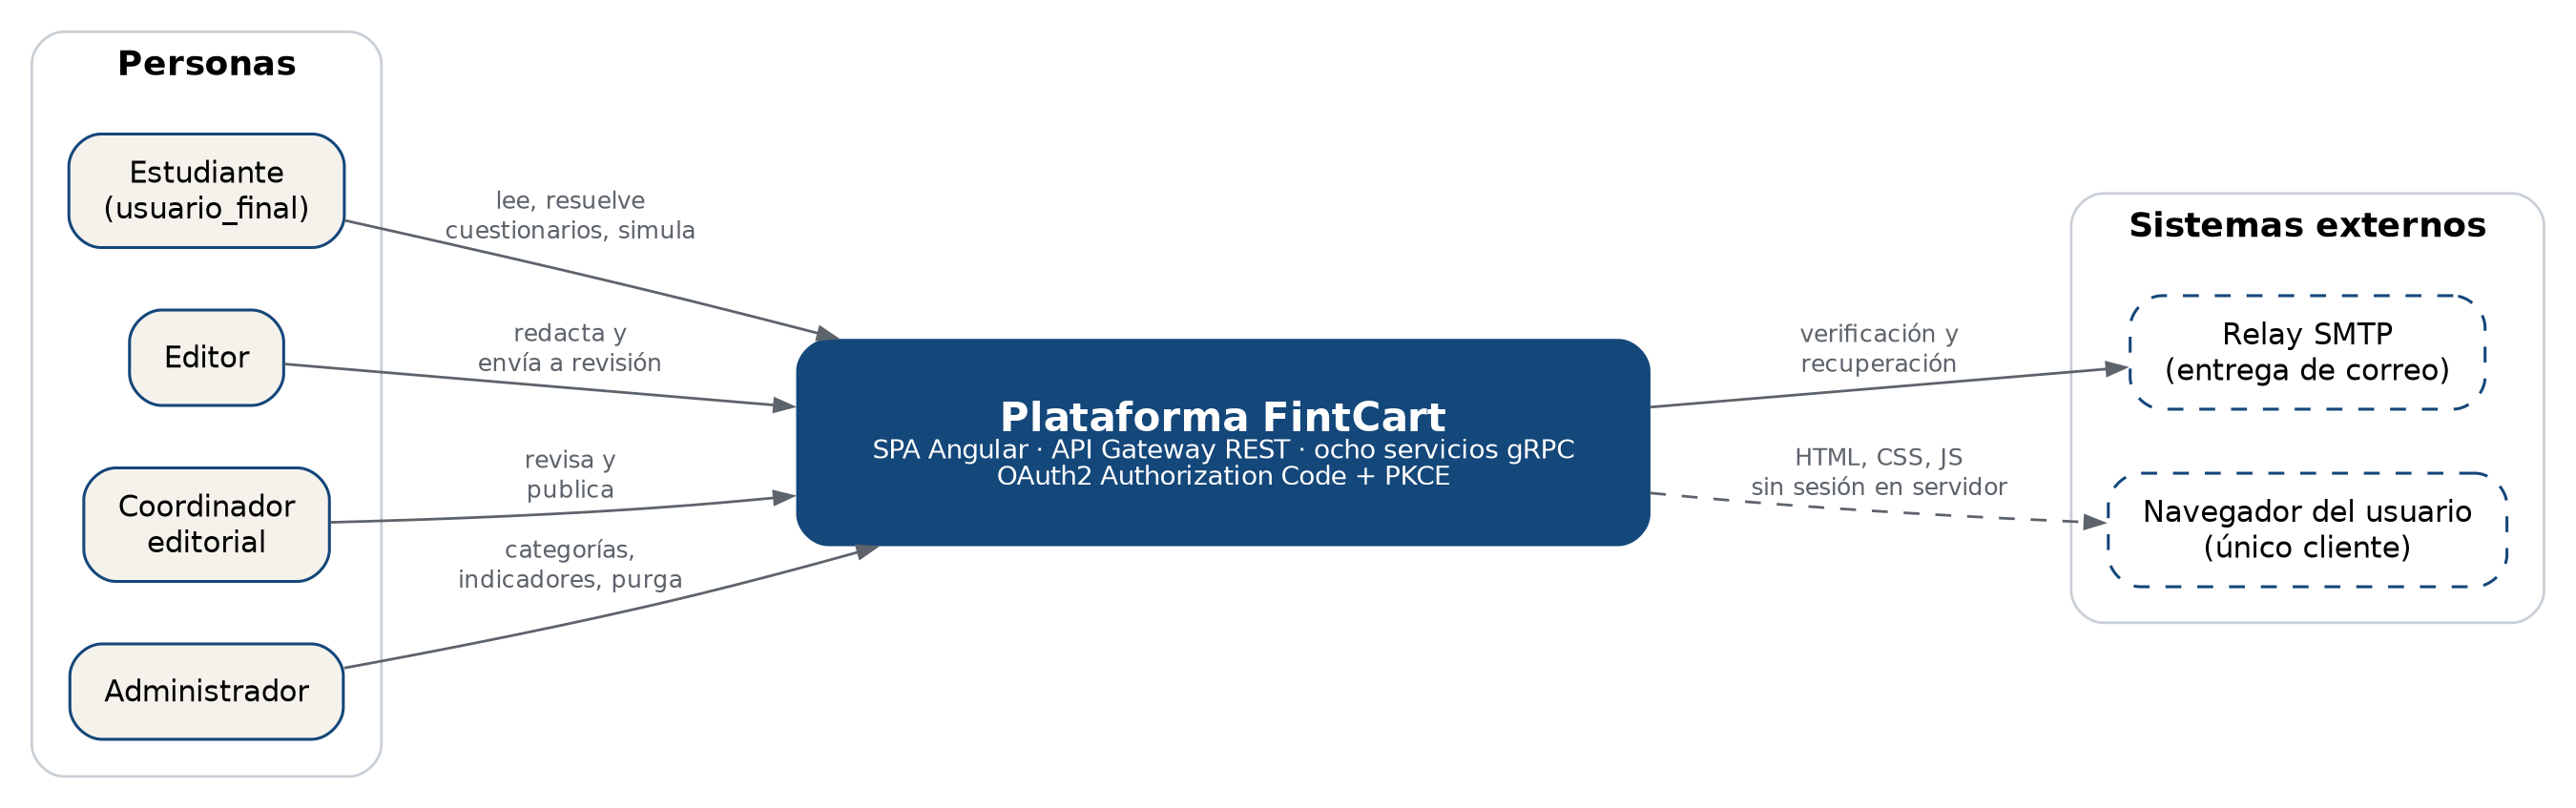
\includegraphics[width=\linewidth]{fig-c4-n1-contexto.png}
  \caption[C4 level 1: system context]{C4 level 1. The platform is one box to the people
  who use it. Everything the reader will later see as a service boundary is invisible here,
  which is the point: the four human roles differ in what they may do, not in what they connect
  to. The relief ``plataforma'' is drawn with the source \code{fig-c4-n1-contexto.dot}.}
  \label{fig:c4-n1}
\end{figure}

Figure~\ref{fig:c4-n1} states the first boundary. A single SPA is the only client;
the Gateway is the only surface that speaks REST; and the two external systems are
a mail relay and the browser itself. The absence of an arrow from person to service
is the architectural claim: no client ever reaches a service directly, so the
Gateway is not a convenience in front of the system but the system's edge.

The table deserves one observation: the four human roles are authorization roles,
not separate client applications. A single SPA serves all of them, and the
distinction between \code{usuario_final}, \code{editor},
\code{coordinador_editorial} and \code{administrador} is carried in the JWT claims
and enforced by role middleware in the Gateway, never by hiding interface
elements in the client (constitution, Principle~VII). The machine-to-machine
actor exists because the platform must be reachable programmatically without a
human session; it uses a different OAuth2 flow but the same Gateway.

\subsection{Containers (C4 level 2)}

The system is decomposed into nine deployable containers: eight backend services
and the SPA. Table~\ref{tab:contenedores} inventories them with their language,
data store and responsibility.

\begin{table}[htbp]
  \centering
  \caption{Container inventory: the eight backend services and the SPA.}
  \label{tab:contenedores}
  \begin{tabular}{@{}l l l p{6.6cm}@{}}
    \hline
    \textbf{Container} & \textbf{Language} & \textbf{Data store} & \textbf{Responsibility} \\
    \hline
    API Gateway & Go 1.24 & none & REST$\leftrightarrow$gRPC translation, rate limiting, role middleware \\
    Auth server & Go 1.24 & PostgreSQL, Redis & OAuth2 flows, JWT issuance and revocation \\
    Orchestrator & Go 1.24 & PostgreSQL & Saga coordination, compensations, periodic sweeps \\
    Users & Go 1.24 & PostgreSQL & Profiles, roles, progress, in-app inbox \\
    Learning & TypeScript, NestJS 11 & PostgreSQL & Articles, versions, quizzes, categories, images \\
    Simulator & Rust 1.85 & PostgreSQL & Formula engine, calculators, indicators, history \\
    Notification & TypeScript, Node & PostgreSQL & E-mail delivery over a persistent queue \\
    Audit & Go 1.24 & PostgreSQL & Immutable, append-only audit log \\
    Frontend SPA & TypeScript, Angular 19 & none & Product surface, OAuth2 PKCE client \\
    \hline
  \end{tabular}
\end{table}

\begin{figure}[htbp]
  \centering
  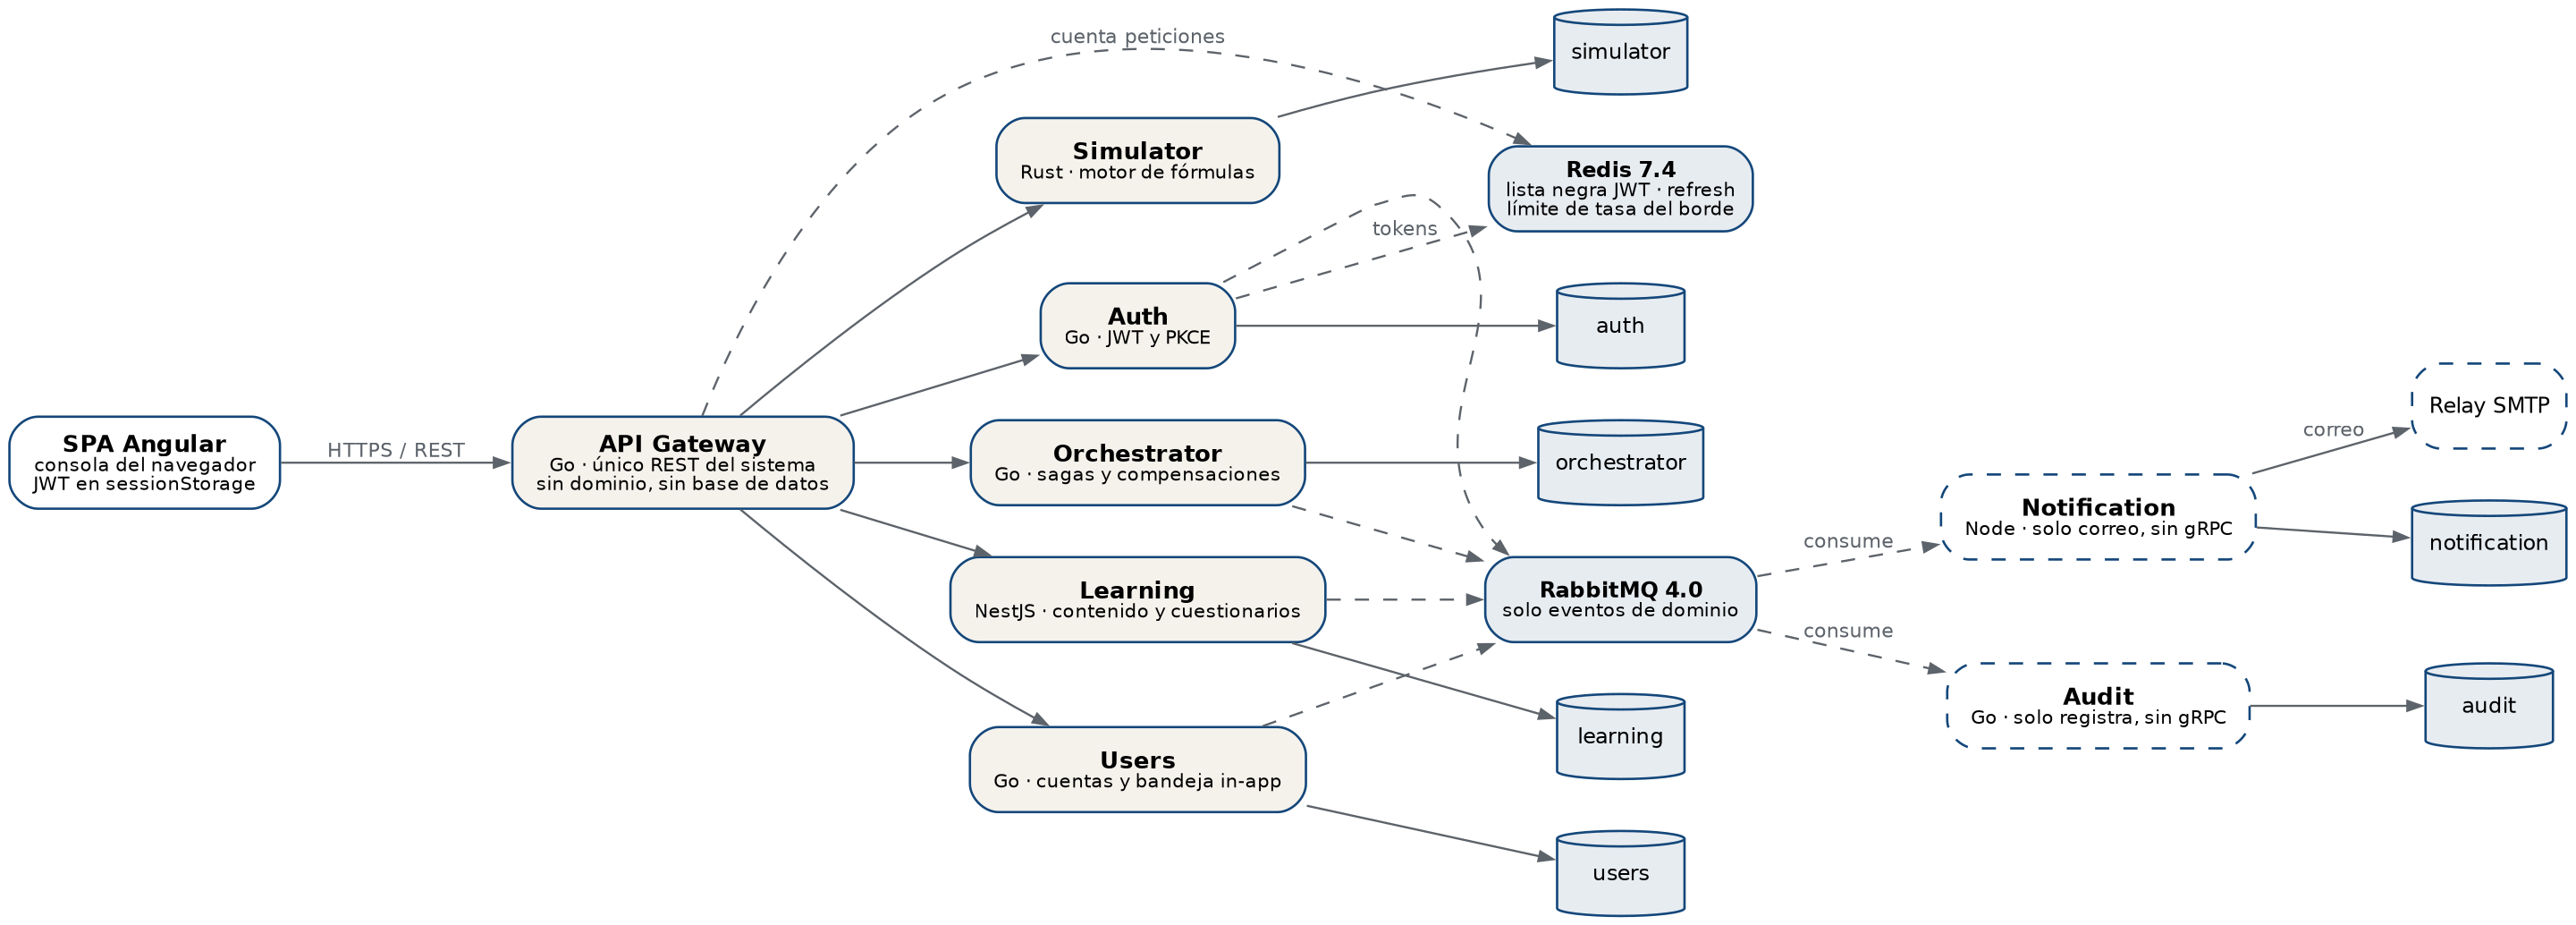
\includegraphics[width=\linewidth]{fig-c4-n2-contenedores.png}
  \caption[C4 level 2: containers]{C4 level 2. The SPA and eight services, seven PostgreSQL
  databases and two pieces of shared infrastructure. The two dashed containers on the right are
  consumers with no gRPC surface: they are degenerate layers under Principle IX, not services that
  forgot to expose an API. Source: \code{fig-c4-n2-contenedores.dot}.}
  \label{fig:c4-n2}
\end{figure}

Figure~\ref{fig:c4-n2} is the diagram that costs the most to defend, because a reader
can count. There are seven databases and no line between them; the two containers on
the right consume events and answer to nobody; and the arrows that carry counts from
\code{Users} to Learning and Simulator are gRPC calls, not joins. The column in the
simulator store that holds a user identifier is deliberately \emph{not} a foreign key:
nothing in this system can enforce a cross-service constraint, so the schema must not
pretend it does.

The language assignment is deliberate, not decorative. Go covers the four
services whose work is transport, coordination and records: the Gateway, the
authentication server, the orchestrator and the users and audit services. Rust is
reserved for the simulator service because that is where the arithmetic lives, and
the non-negotiable precision rule is easiest to enforce in a language whose type
system can forbid floating point at compile time. NestJS hosts the learning
service, where the domain is document-shaped and the team benefits from a typed
framework; plain Node is enough for the notification service, which has no gRPC
surface and does one thing well. The reasons for separation are those the pattern
itself promises: \textcite{dhandapani2025microservices} argues that financial
systems move from monoliths to microservices to gain real-time processing,
scalability and resilience on domain-driven boundaries, and
\parencite{miao2020microservice} describe the same decomposition in an
educational platform. The pedagogical migration of a legacy insurance core that
\textcite{lange2019microservices} report shows the cost side: the boundaries are
bought with operational complexity, which here is paid once and codified as rules.

Each stateful service owns its own PostgreSQL 16 database, and no service may
read another service's database (constitution, Principle~III). There are seven
such databases; the Gateway and the SPA hold none. Redis 7.4 appears in exactly
two places: the authentication server keeps the JWT blacklist and refresh tokens
there, and the Gateway keeps its distributed rate-limit counters there
(Principle~IV). RabbitMQ 4.0 carries events from the four producers --- users,
learning, orchestrator and authentication --- exclusively to the two pure
consumers, notification and audit (Principle~V). The simulator service is
deliberately absent from the producer list: it never publishes, so its
simulation audit events are emitted by the orchestrator on its behalf.

Two services do not instantiate the full three-layer shape, and that is a
constitution argument rather than an oversight. The Gateway has no domain and no
database: it is pure transport plus outgoing gRPC clients and rate limiting.
Notification and audit are pure consumers with no gRPC server, so their transport
layer is the AMQP consumer. The plan records these as legitimate degenerate
layers (\code{specs/001-fintcart-platform/plan.md:240-243}), and treating them as
complete stacks would be an anti-pattern: it would add a \code{server} layer with
nothing to serve.

\subsection{Components (C4 level 3)}

Two components carry the thesis and are worth opening: the formula engine inside
the simulator service, and the publishing and content flow inside the learning
service. Both are described at the level of their internal modules, under the
layering rule of Principle~IX.

\textbf{The formula engine.} The simulator service is no longer a closed set of
wired calculators; it is a formula engine that turns a parameterized definition
into a computed result. A calculator is data --- an identity row plus the
immutable definition version it serves --- while the engine is the code that
parses, stores and evaluates that definition. The engine has three stages and a
boundary. A lexer turns the author's text into tokens; a parser validates the
expression at save time and produces an abstract syntax tree (AST); the AST is
persisted as \code{JSONB}; and a bounded evaluator walks the tree in
\code{rust_decimal}. Text is never parsed at execution time and code is never
executed (\code{services/simulator/src/domain/formula/mod.rs:1-25}). The AST is
bounded by construction: a definition may have at most 20 inputs and 10 outputs,
each formula at most 64 nodes and depth 16, checked before persistence, so the
evaluator needs no runtime watchdog (\code{services/simulator/src/domain/formula/limits.rs:24-33}).
Two functions are kept apart on purpose: \code{pot} raises to an integer exponent
by repeated multiplication and is exact, while \code{potd} raises to a decimal
exponent through transcendental functions and is approximate. Fusing them would
silently lose the exactness that Principle~VIII exists to protect.

The engine respects the layering rule exactly. Its modules live under
\code{src/domain/formula/} and import neither transport types nor database rows:
the lexer, parser, AST, evaluator and limits are pure domain code. The transport
layer is \code{src/grpc/service.rs}, and the only place where a decimal
\code{string} from the wire becomes a \code{Decimal} --- and back --- is
\code{src/grpc/mapping.rs}. That confinement is the point of the mapping layer:
the three representations (transport DTO, domain type, database row) are distinct
by rule (Principle~IX), and the decimal conversion, the single highest-risk
operation in the system, happens in exactly one module per boundary.

\textbf{The publishing and content flow.} Inside the learning service, an
article body stopped being plain text and became a block document: the
\code{article_versions.body_doc} column holds a \code{JSONB} tree with a closed
vocabulary of nodes --- \code{doc}, \code{parrafo}, \code{encabezado},
\code{lista}, \code{item_lista}, \code{texto}, \code{imagen} and
\code{calculadora} --- and a closed set of marks: \code{negrita}, \code{cursiva}
and \code{enlace}. No HTML is persisted anywhere. Validation is positive and
server-side: the validator enumerates what is admitted and rejects everything
else, including any link whose scheme is not \code{http}, \code{https} or
\code{mailto} (\code{services/learning/src/articles/body-doc.validator.ts:1-20}).
Because the body is a tree of typed blocks, the frontend renders each node with a
component and never calls \code{innerHTML}, so there is no injection surface to
sanitize. The publishing flow (\code{src/publishing/}) sits in the application
layer, and the gRPC controller plus its mapping module in the transport layer
(\code{src/grpc/}); the repository is the only layer that emits SQL.

\begin{figure}[htbp]
  \centering
  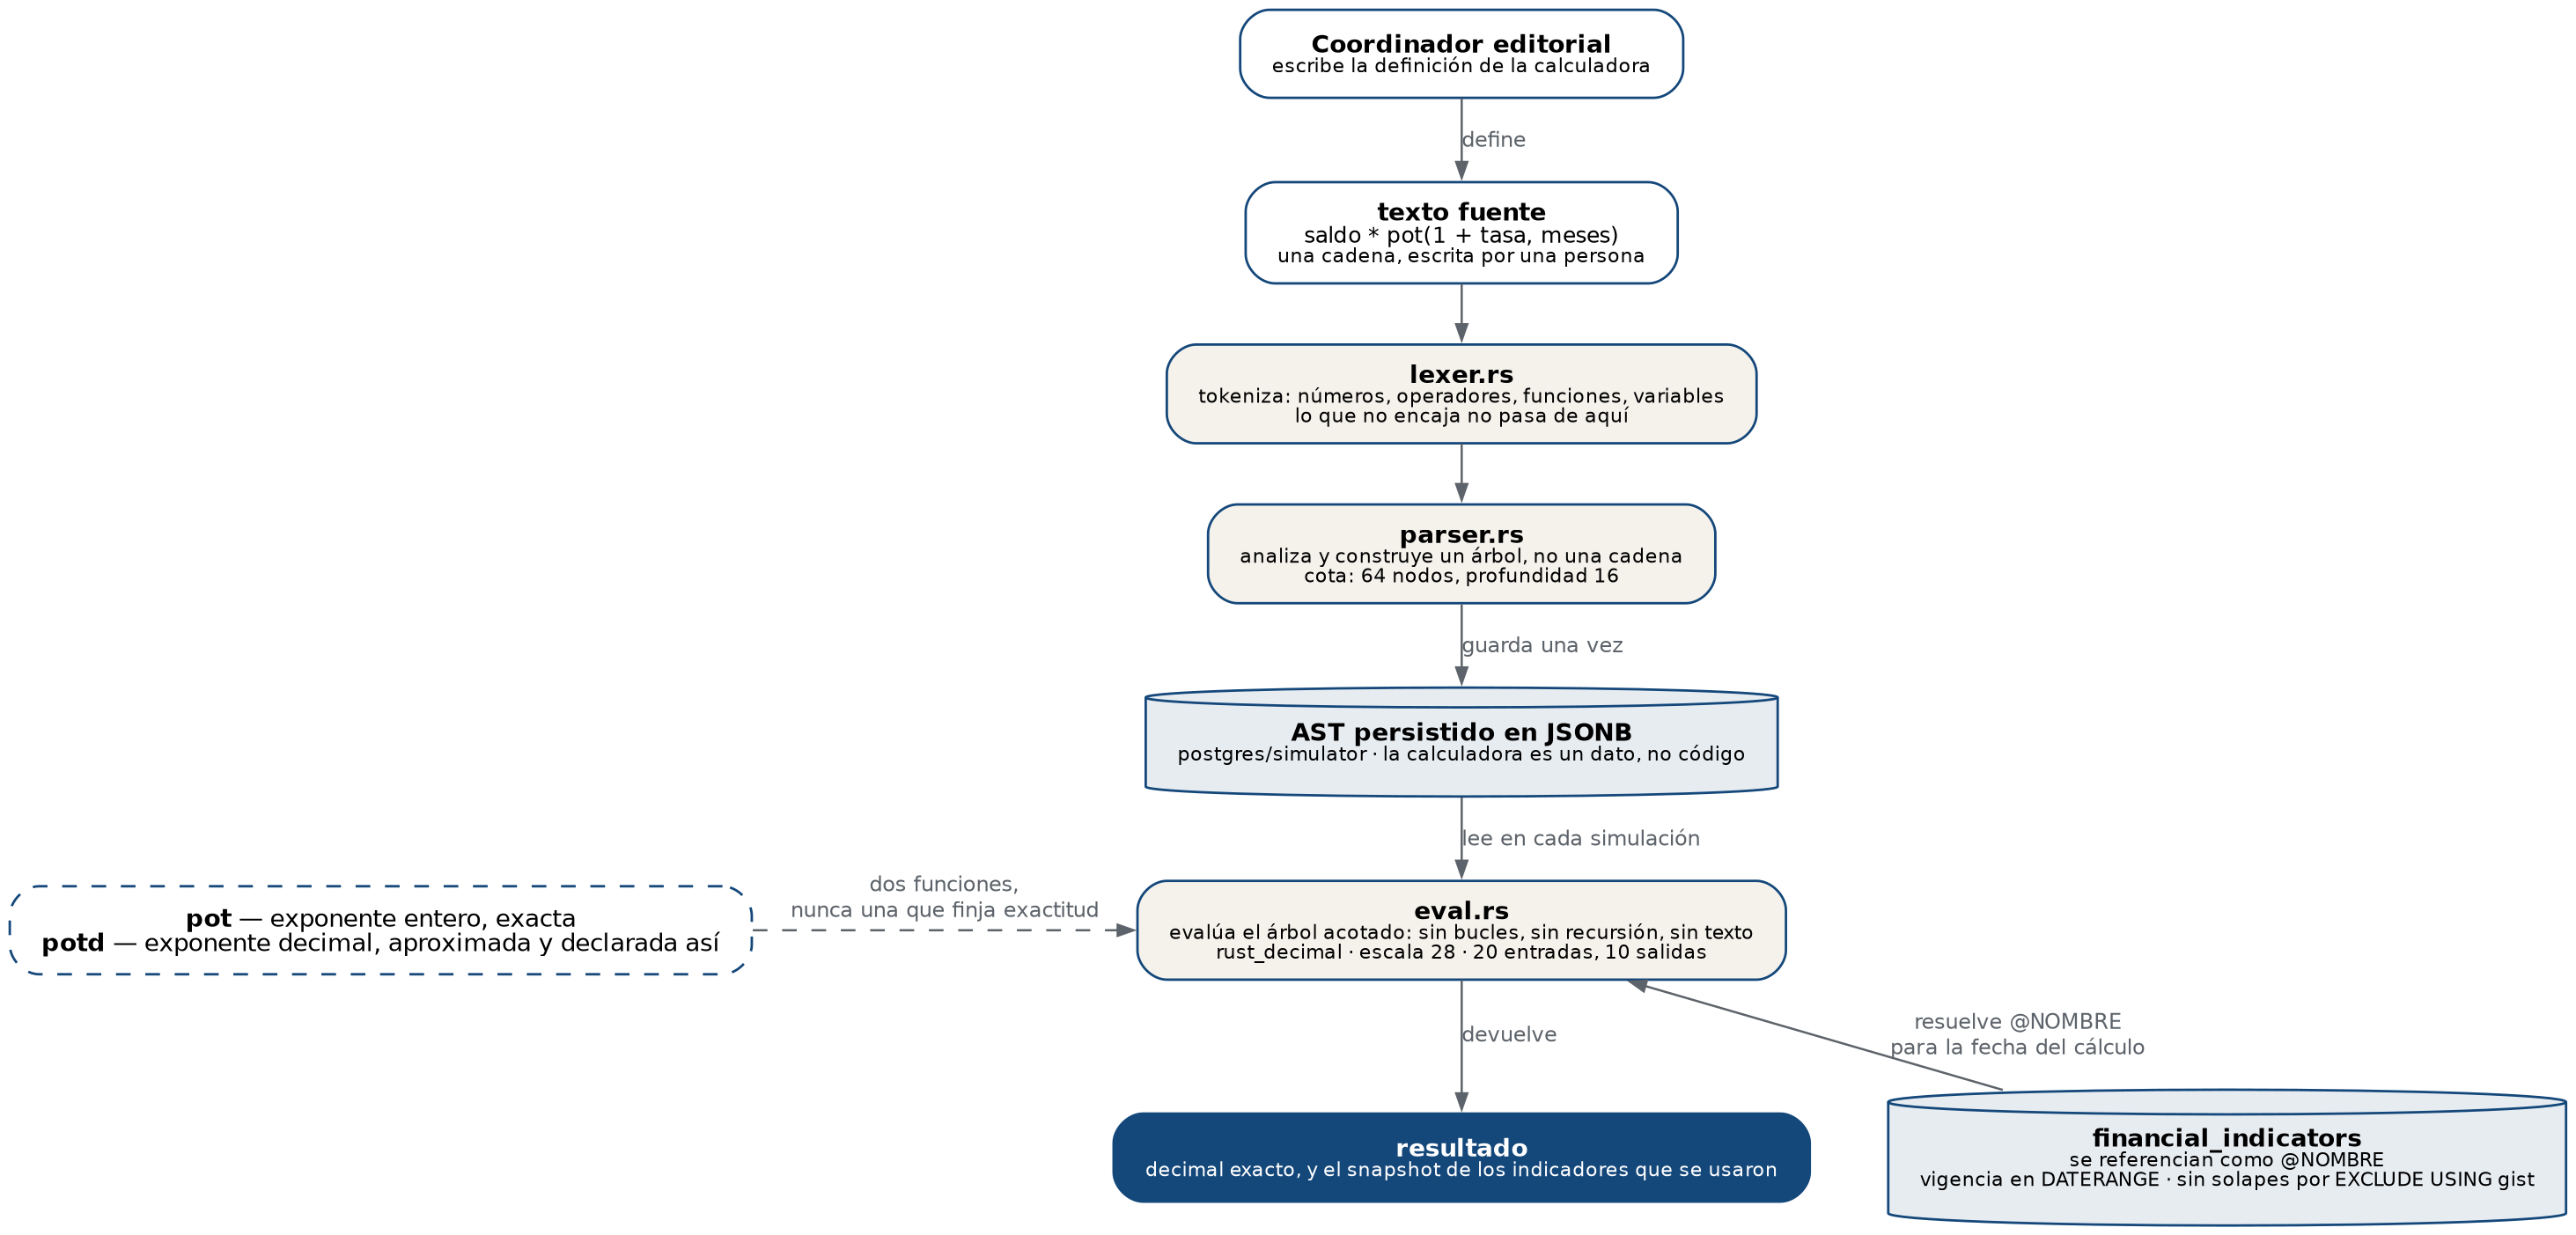
\includegraphics[width=0.92\linewidth]{fig-c4-n3-motor-formulas.png}
  \caption[C4 level 3: the formula engine]{C4 level 3, first flow. A calculator is a row, not
  a build artifact: the source text becomes a tree once, and every simulation then evaluates
  that tree. \code{pot} and \code{potd} are separate because merging them would silently trade
  exactness for convenience. Source: \code{fig-c4-n3-motor-formulas.dot}.}
  \label{fig:c4-n3-motor}
\end{figure}

\begin{figure}[htbp]
  \centering
  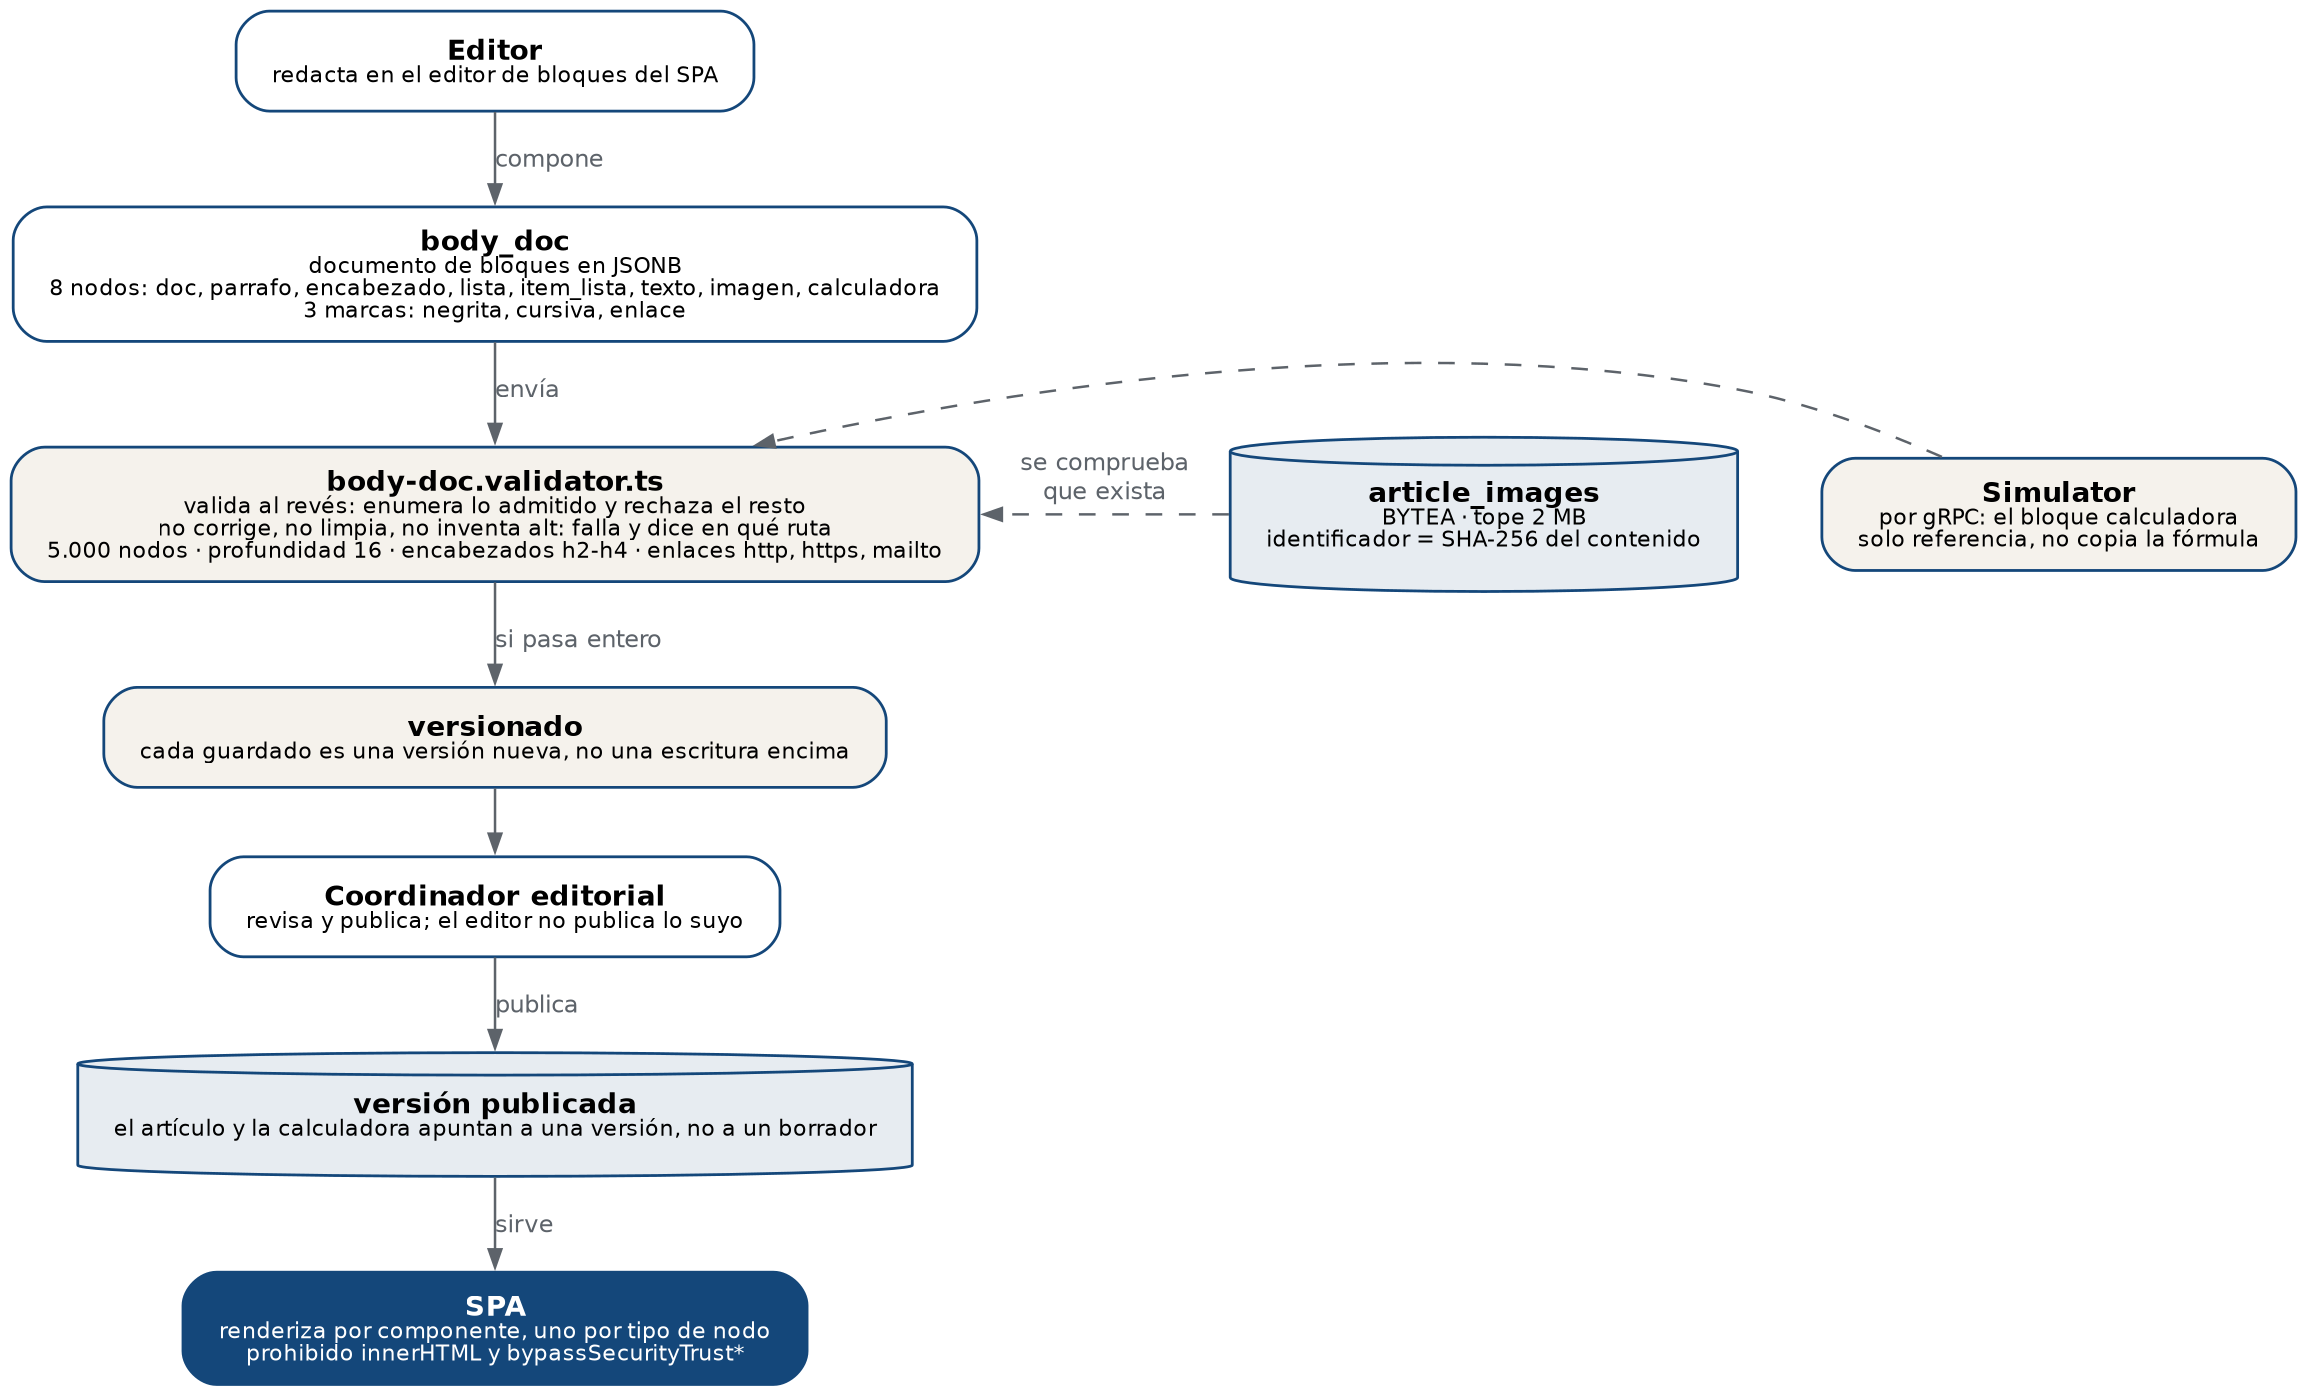
\includegraphics[width=0.92\linewidth]{fig-c4-n3-publicacion.png}
  \caption[C4 level 3: publishing]{C4 level 3, second flow. The validator is negative by design:
  it enumerates what is admitted and rejects the rest, reporting the path to the offending node
  instead of repairing it. The SPA renders one component per node type and never interprets HTML.
  Source: \code{fig-c4-n3-publicacion.dot}.}
  \label{fig:c4-n3-publicacion}
\end{figure}

Figures~\ref{fig:c4-n3-motor} and~\ref{fig:c4-n3-publicacion} open the two components
whose internals decide whether the rest of the design holds. Both are pipelines with a
narrow waist: in the first the waist is the persisted AST, in the second it is the block
vocabulary. In each case the expensive guarantee -- exact decimal arithmetic in one,
no injection surface in the other -- is obtained by making the input smaller and
rejecting it early, not by checking the output afterwards.

\subsection{Architecture decisions}

The planning phases recorded decisions D-13 through D-32; this section promotes
them to ADRs. Table~\ref{tab:adrs} is the index, grouped by the area each
decision governs.

\begin{table}[htbp]
  \centering
  \caption{ADR index for decisions D-13 through D-32, grouped by area.}
  \label{tab:adrs}
  \begin{tabular}{@{}l l p{8.6cm} l@{}}
    \hline
    \textbf{Area} & \textbf{ID} & \textbf{Decision} & \textbf{Source} \\
    \hline
    Content & D-13 & Article images stored as \code{BYTEA}, content-addressed by SHA-256 & 002 research.md:13-64 \\
    Content & D-14 & Article body as a \code{JSONB} block document with a closed vocabulary & 002 research.md:66-123 \\
    Content & D-24 & TipTap as the writing-surface editor; its document model equals D-14 & 002 research.md:379-400 \\
    Formula engine & D-15 & Closed grammar, AST validated and persisted at save, bounded evaluation & 002 research.md:125-184 \\
    Formula engine & D-16 & Native calculators re-seeded as platform seed definitions & 002 research.md:186-227 \\
    Quizzes & D-17 & Quiz session stored in \code{learning_db} with 60-minute validity & 002 research.md:229-247 \\
    Quizzes & D-18 & \code{score} becomes a percentage over 100 & 002 research.md:249-275 \\
    Administration & D-19 & Category catalog replaces the free-text \code{category} column & 002 research.md:277-294 \\
    Administration & D-20 & Purge grace period executed by the orchestrator's sweep & 002 research.md:296-323 \\
    Administration & D-21 & \code{administrador} role propagation and idempotent bootstrap & 002 research.md:325-341 \\
    Administration & D-22 & Yearly indicators owned by the simulator, snapshotted per simulation & 002 research.md:343-364 \\
    Administration & D-23 & Indicator expiry alert published by the orchestrator & 002 research.md:366-377 \\
    Integration & D-25 (feature 002) & Embedded calculators run the normal simulation path & 002 research.md:402-416 \\
    Simulator & D-26 (feature 002) & Sixth \code{calc_type} value for user-defined calculators & 002 research.md:419-448 \\
    Simulator & D-27 (feature 002) & Annuity overflow panics corrected after the regression baseline & 002 research.md:450-472 \\
    Simulator & D-28 (feature 002) & Seed definitions deployed as an explicit step, not at startup & 002 research.md:474-518 \\
    Simulator & D-29 (feature 002) & Seed runs recorded with their native \code{calc_type} & 002 research.md:520-555 \\
    Simulator & D-30 (feature 002) & Native code retirement order & 002 research.md:557-601 \\
    Frontend & D-26 (feature 003) & Remove the handcrafted style layer rather than add one & 003 research.md:12-39 \\
    Frontend & D-27 (feature 003) & Four breakpoints declared as design tokens & 003 research.md:41-80 \\
    Frontend & D-28 (feature 003) & Screen-by-screen migration grouped by UI kit & 003 research.md:82-109 \\
    Frontend & D-29 (feature 003) & Existing end-to-end suites kept as the regression net & 003 research.md:111-161 \\
    Frontend & D-30 (feature 003) & App shell treated as a twentieth surface & 003 research.md:163-178 \\
    Frontend & D-31 & Marketing landing kept out of scope & 003 research.md:180-193 \\
    Frontend & D-32 & Shared loading, empty and error components; money never truncates & 003 research.md:195-219 \\
    \hline
  \end{tabular}
\end{table}

The reader will notice that the collision spans six identifiers, D-25 through
D-30. The \code{002} plan defines D-13 through D-30 and the \code{003} plan
defines D-26 through D-32, so D-26 through D-30 name a different decision in each
feature, while D-25 is the boundary that the \code{003} plan assumed \code{002}
had stopped at and that \code{002} later crossed. The index and the headings
therefore cite all six feature-qualified, so that no reader follows the wrong
ADR, and this collision is reported as a finding rather than resolved silently.

The decisions themselves, in standard form, grouped as in the table.

\textbf{Content.} D-13: context --- article illustrations needed storage on a
deployment of two 4\,GB VPSs that already runs seven databases, Redis, RabbitMQ
and eight services, where an object store would demand a constitutional amendment.
Decision --- store images as \code{BYTEA} in \code{learning_db} with
\code{STORAGE EXTERNAL}, a 2\,MB cap, and the SHA-256 of the bytes as identifier.
Consequences --- backups stay a single \code{pg_dump}, versions share immutable
rows, and the repository interface leaves an object store as a later swap without
touching domain or contract. D-14: context --- the enriched body had to be
safe-by-construction, not safe-by-sanitizer. Decision --- a \code{JSONB} block
document with a closed vocabulary validated in the server at save time.
Consequences --- the frontend renders per node with no \code{innerHTML} surface,
and deny-by-default validation is stronger than cleaning arbitrary HTML. D-24 is
the client half of D-14: TipTap's document model already is the block tree, so
there is no translation layer in which attributes could be lost, and the client
schema is explicitly not the validation.

\textbf{Formula engine.} D-15: context --- calculators had to accept author
formulas without executing code or hanging the service. Decision --- a closed
grammar, parsed at save, AST persisted, bounded evaluation in
\code{rust_decimal}; loops, recursion and text values are forbidden.
Consequences --- errors surface while editing, cost is bounded by construction,
and persisting the AST freezes published formulas against silent
reinterpretation. D-16: context --- the five original calculators had to survive
the migration. Decision --- they are reproducible and are re-seeded as platform
seed definitions over the same engine. Consequences --- the seed regression suite
is the gate that keeps the native code alive until the engine matches it
result for result. One count is worth stating in the prose: the code ships ten
seed definitions (\code{services/simulator/src/domain/seeds/mod.rs:144-155}),
because three further calculators (\code{fondo_emergencia}, \code{meta_ahorro},
\code{cdt_dias}) were added after the spec was written and the plan text was never
updated --- the spec is one count behind the code it describes, and the code is
what runs.

\textbf{Quizzes.} D-17: context --- the quiz session is ephemeral state that looks
like a cache candidate. Decision --- it lives in \code{learning_db} with
60-minute validity, because Redis is constitutionally confined and business
session state is prohibited there. Consequences --- the session survives in the
database until purged, and the attempt history is not left depending on a cache.
D-18: context --- the score was an absolute weighted sum. Decision --- it becomes
a percentage over 100, with the historical migration rewriting existing scores.
Consequences --- the migration is exact only where the question bank did not
change, and that residual approximation is counted and reported rather than
hidden.

\textbf{Administration.} D-19 replaces the free-text category with a catalog that
is never physically deleted. D-20 assigns the purge sweep to the orchestrator,
which asks users over gRPC which accounts are due and reuses the existing
anonymization saga. D-21 adds the \code{administrador} role through the role
claims and a Gateway middleware, and bootstraps the first administrator from an
environment variable so that no privileged user is written into a migration.
D-22 keeps yearly indicators in the simulator, the only consumer of their value,
and snapshots the values used into every simulation so history remains
explicable after an indicator changes. D-23 has the orchestrator publish the
indicator-expiry alert, preserving the rule that the simulator never produces
events.

\textbf{Integration.} D-25 (feature 002): an embedded calculator in an article runs exactly the
normal simulation path --- Gateway, orchestrator, simulator --- so it lands in
the history and the audit trail like any other simulation, and the article only
contributes the opaque \code{calculator_id}.

\textbf{Simulator corrections (feature 002).} D-26 (feature 002) records a user-defined calculator's
simulation with a sixth \code{calc_type} value (\code{usuario}), keeping the
column \code{NOT NULL} and meaning what it says. D-27 (feature 002) defers the correction of
annuity overflow panics until after the regression baseline is frozen, so the
reference is not modified while it is being measured. D-28 (feature 002) makes seed deployment
an explicit, idempotent step rather than a startup side effect, keeping the
entrypoint thin. D-29 (feature 002) records a seed run under the native type it reproduces,
so the history does not call a platform seed a user calculator. D-30 (feature 002) orders the
retirement of the native code so that the domain never depends on the code being
removed and the compatibility path is redirected only after the production seed
step exists.

\textbf{Frontend redesign (feature 003).} D-26 (feature 003) removes the handcrafted style layer instead of
adding a third one, with its deletion as the measurable completion criterion.
D-27 (feature 003) defines four breakpoints (480, 768, 1024, 1280\,px) as design tokens with a
360\,px minimum, because no responsive behavior existed anywhere. D-28 (feature 003) migrates
screen by screen grouped by UI kit so the editorial kit --- the only overlap with
\code{002} --- lands last. D-29 (feature 003) keeps the existing end-to-end suites untouched
because they select by role and accessible label and therefore double as an
accessibility regression net. D-30 (feature 003) folds the app shell, visible in every view,
into the scope. D-31 keeps the marketing landing out. D-32 derives the loading,
empty and error states as shared components and fixes the rule that a monetary
figure never truncates, because a truncated figure is a false datum.

\subsection{Constitutive tensions}

Four tensions are structural, and the design refuses to resolve them by
convenience.

\textbf{gRPC inside, REST only at the edge.} Internal communication is gRPC with
Protocol Buffers, and REST/HTTP exists only at the Gateway. The asymmetry is
not a stylistic preference: gRPC gives typed, checked contracts and better
performance for the high-frequency internal calls, while REST at the edge keeps
the public surface compatible with standard web clients. The cost is a permanent
translation duty concentrated in the Gateway, which is precisely why the Gateway
is allowed to be a transport-only degenerate layer.

\textbf{Decimal precision as a non-negotiable.} Money, rates and simulation
results are represented with arbitrary-precision decimals in every layer, and
binary floating point is forbidden everywhere. The rule names the representation
per technology: \code{NUMERIC} columns in PostgreSQL,
\code{shopspring/decimal} in Go, \code{rust_decimal} in Rust,
\code{decimal.js}/\code{big.js} in TypeScript, and the canonical decimal
\code{string} in Protocol Buffers and JSON. The simulator service enforces this at
the type level, denying \code{f32}/\code{f64} across the crate. This is the
Principle~VIII that the formula engine, the mapping layers and the never-truncate
rule of D-32 all exist to serve.

\textbf{No two-phase commit; sagas with compensation.} Any operation that crosses
two or more services is a saga coordinated by the orchestrator, with an explicit
compensation per step; two-phase commit and distributed locks are prohibited. The
orchestrator holds no domain logic of its own --- it sequences steps and runs
compensations --- and the periodic sweeps of D-20 and D-23 are sequencing, not
domain rules. The trade is eventual consistency bought with auditable
compensation instead of a distributed transaction, which the constitution judges
the right price for the decoupling it buys.

\textbf{The membership oracle (FR-077).} When an account is anonymized, the
system keeps no representation of the original e-mail address --- not even
transformed or encrypted. The reason is not storage economy: a hash of an e-mail
address is a membership oracle, because address spaces are enumerable and
low-entropy, so anyone with the table could test whether a specific person ever
held an account, reintroducing exactly the re-identification the anonymization
destroys. The design routes the owner's address to the notification e-mail
through a routing key that never reaches the immutable audit log, so the audit
retention of five years cannot become a backdoor to the address.
